\chapter{Estabilidade do genoma: dano, reparo e recombinação do DNA}\label{ch:b3:dna-repair}

Uma tarde de praia deposita umas cem mil lesões químicas no DNA de
cada célula da pele exposta ao sol: timinas adjacentes soldadas em
dímeros pela luz ultravioleta, bases oxidadas, fitas cortadas. Sem sol
algum, a água morna da célula arranca cerca de dez mil purinas de seus
açúcares por dia e converte centenas de citosinas em uracila. Ainda
assim, a taxa de mutação de uma célula humana é de cerca de uma
mudança em dez bilhões de pares de bases por divisão --- num genoma de
seis bilhões, menos de uma mutação nova por divisão. A distância entre
o dano que um genoma sofre e o dano que ele conserva é fechada pelo
reparo: uma dúzia de sistemas enzimáticos que patrulham a
dupla-hélice, reconhecem o que não deveria estar ali, recortam-no e
reconstroem a partir da fita intacta e, quando as duas fitas estão
quebradas, as reúnem ou copiam o pedaço que falta de uma irmã. As
crianças que não têm um desses sistemas --- que se queimam ao primeiro
toque de sol, ou que desenvolvem câncer de cólon aos trinta anos ---
mostram quanto os sistemas valem. Este capítulo trata do dano, das
vias de reparo, da maquinaria de recombinação que repara as piores
quebras e que a meiose toma emprestada, e da decisão da célula,
quando o reparo falha, de parar de se dividir ou de morrer.

\section{O que dá errado no DNA}

\begin{definition}[Lesões do DNA]\label{def:b3:dna-repair:lesions}
\index{lesão do DNA}\index{depurinação}\index{desaminação}\index{dímero de pirimidina}\index{quebra de fita dupla}\index{8-oxoguanina}
Uma \emph{lesão} é qualquer alteração química do DNA que o afaste das
quatro bases normais corretamente pareadas sobre um esqueleto intacto.
As lesões espontâneas vêm da química da água e do oxigênio: a
\emph{depurinação}, hidrólise da ligação entre uma purina e seu
açúcar, que deixa um sítio abásico (cerca de $10^{4}$ por célula por
dia); a \emph{desaminação}, que converte a citosina em uracila, a
5-metilcitosina em timina e a adenina em hipoxantina (algumas centenas
por dia); a \emph{oxidação} por espécies reativas de oxigênio,
sobretudo a \emph{8-oxoguanina}, que pareia com a adenina tão
prontamente quanto com a citosina; e os \emph{erros de replicação},
uma base mal incorporada ou deslizada. Entre as lesões ambientais
estão o \emph{dímero ciclobutânico de pirimidina} e o fotoproduto 6-4
feitos pela luz ultravioleta entre duas pirimidinas adjacentes; as
bases alquiladas por agentes alquilantes (a O$^{6}$-metil-guanina
pareia com a timina); os adutos volumosos de hidrocarbonetos
aromáticos e da aflatoxina; as ligações cruzadas entre fitas da
cisplatina e das mostardas nitrogenadas; e as quebras de fita simples
e de \emph{fita dupla} feitas pela radiação ionizante, cerca de
\num{1000} quebras de fita simples e \numrange{30}{40} de fita dupla
por célula por gray.
\end{definition}

\begin{proposition}[A escada da fidelidade]\label{prop:b3:dna-repair:fidelity}
\index{fidelidade}\index{revisão}\index{reparo de mau pareamento}
A replicação alcança sua taxa de erro de cerca de $10^{-10}$ por par
de bases em três etapas multiplicativas. A seleção da base pela
polimerase, pela geometria e pelas pontes de hidrogênio, erra cerca de
uma vez em $10^{5}$; a \emph{revisão} pela exonuclease
3$'\to$5$'$ da polimerase, que excisa uma base terminal mal pareada
antes da extensão, remove \qty{99}{\%} desses erros; o \emph{\omterm{prop:b3:dna-repair:fidelity}{reparo de
mau pareamento}}, agindo atrás da forquilha sobre a fita recém-feita,
remove \qty{99.9}{\%} do que resta. O produto
$10^{-5}\times 10^{-2}\times 10^{-3} = 10^{-10}$ é a taxa observada, e
um defeito em qualquer das etapas de correção a eleva cem ou mil
vezes: tais células são \emph{mutadoras}.
\end{proposition}

\begin{example}[Lesões contra mutações]\label{ex:b3:dna-repair:numbers}
Uma célula humana de $6.4\times 10^{9}$ pares de bases que se divide
uma vez por dia acumula da ordem de $10^{4}$--$10^{5}$ lesões por dia
e cerca de $6.4\times 10^{9}\times 10^{-10} \approx 0.6$ mutações
novas por divisão: menos de uma \omterm{def:b3:dna-repair:lesions}{lesão} em dez mil sobrevive para se
tornar uma mudança permanente. As demais são reparadas antes que a
replicação as leia, e é a taxa de sobrevivência até a mutação --- e
não a taxa de dano --- que a seleção minimizou. A mesma aritmética
mostra por que o número de mutações num tumor ou no esperma de um pai
mais velho conta divisões: as mutações que uma célula carrega são, em
primeira ordem, as divisões que ela sofreu vezes o erro por divisão.
\end{example}

\section{Reparo de uma fita danificada}

\begin{definition}[Reparo por excisão]\label{def:b3:dna-repair:excision}
\index{reparo por excisão de bases}\index{reparo por excisão de nucleotídeos}\index{glicosilase}\index{xeroderma pigmentoso}
A maioria das lesões afeta uma só fita e é reparada recortando o
pedaço danificado e copiando a outra fita. O \emph{reparo por excisão
de bases} (BER) cuida de lesões pequenas que não distorcem a hélice:
uma \emph{DNA-glicosilase} específica para um tipo de base errada
(uracila-DNA-glicosilase, glicosilase da 8-oxoG e várias outras) vira
a base para fora da hélice e a corta de seu açúcar; uma AP-endonuclease
corta o esqueleto no sítio abásico; uma polimerase (a Pol~$\beta$)
remove o açúcar e insere um nucleotídeo; uma ligase sela. O
\emph{reparo por excisão de nucleotídeos} (NER) cuida de lesões
volumosas que distorcem a hélice --- \omterm{def:b3:dna-repair:lesions}{dímeros de pirimidina}, adutos
químicos --- sem reconhecer a química da \omterm{def:b3:dna-repair:lesions}{lesão} em si: a distorção é
detectada (pela XPC que varre o genoma, ou por uma RNA-polimerase
parada, no ramo acoplado à transcrição), a hélice é aberta pelas
subunidades helicase do TFIIH, o dano é verificado (XPA), duas
endonucleases (XPF, XPG) cortam a fita danificada a
\numrange{24}{32} nucleotídeos de distância, o oligonucleotídeo é
liberado, e a polimerase e a ligase preenchem a lacuna. A perda de
qualquer uma das sete proteínas XP causa o \emph{xeroderma
pigmentoso}: sensibilidade extrema à luz do sol, sardas e uma taxa mil
vezes maior de câncer de pele.
\end{definition}

\begin{proof}[Evidência]
Cleaver (1968) cultivou fibroblastos de pele de pacientes com
\omterm{def:b3:dna-repair:excision}{xeroderma pigmentoso}, irradiou-os com luz ultravioleta e lhes deu
timidina radioativa fora da fase S. As células normais incorporaram a
marcação em muitos sítios pequenos --- a ``síntese de DNA não
programada'' dos remendos de reparo ---, ao passo que as células dos
pacientes quase nada incorporaram e morreram em doses que as normais
sobreviviam: a doença é uma falha em excisar os dímeros. Fundir
células de dois pacientes muitas vezes restaurava o reparo no híbrido,
cada célula fornecendo o que faltava à outra; por esse teste os
pacientes foram separados em grupos de complementação, de A a G, um
por gene da via, anos antes de os genes serem clonados.
\end{proof}

\begin{omfigure}
\begin{tikzpicture}[every node/.style={font=\scriptsize}, >=stealth]
  % BER column
  \node[font=\small\bfseries] at (2.0,3.2) {Reparo por excisão de bases};
  \foreach \y/\txt in {2.6/{base danificada (U, 8-oxoG)}, 1.5/{a glicosilase remove a base}, 0.4/{a AP-endonuclease corta}, -0.7/{a Pol $\beta$ preenche um nucleotídeo, a ligase sela}} {
    \draw[very thick, omDef] (0.2,\y) -- (3.8,\y); \draw[very thick, omDef] (0.2,\y-0.25) -- (3.8,\y-0.25);
    \node[right, align=left] at (0.2,\y-0.6) {\txt};
  }
  \fill[omThm] (2.0,2.6) circle (0.1);
  \draw[omThm, thick] (1.9,1.5) -- (2.1,1.5);
  \draw[white, very thick] (1.9,0.4) -- (2.1,0.4);
  \fill[omMeth!80!black] (2.0,-0.7) circle (0.1);
  % NER column
  \node[font=\small\bfseries] at (8.0,3.2) {Reparo por excisão de nucleotídeos};
  \foreach \y/\txt in {2.6/{lesão volumosa distorce a hélice; a XPC se liga}, 1.5/{o TFIIH abre a hélice, a XPA verifica}, 0.4/{XPF e XPG cortam a 24--32 nt de distância}, -0.7/{a polimerase preenche a lacuna, a ligase sela}} {
    \draw[very thick, omDef] (6.2,\y) -- (9.8,\y); \draw[very thick, omDef] (6.2,\y-0.25) -- (9.8,\y-0.25);
    \node[right, align=left] at (6.2,\y-0.6) {\txt};
  }
  \draw[omThm, very thick] (7.8,2.6) -- (8.2,2.6) -- (8.2,2.75) -- (7.8,2.75) -- cycle;
  \draw[omDef, very thick] (7.2,1.5) .. controls (7.6,1.85) and (8.4,1.85) .. (8.8,1.5); \draw[omThm, very thick] (7.85,1.72) -- (8.15,1.72);
  \draw[very thick, white] (7.0,0.4) -- (9.0,0.4); \draw[omThm, thick, ->] (7.0,0.7) -- (7.0,0.48); \draw[omThm, thick, ->] (9.0,0.7) -- (9.0,0.48);
  \draw[very thick, omMeth!80!black] (7.0,-0.7) -- (9.0,-0.7);
\end{tikzpicture}

{\small Duas vias de excisão. A excisão de bases (à esquerda)
reconhece uma base errada específica com uma \omterm{def:b3:dna-repair:excision}{glicosilase} dedicada e
troca um nucleotídeo. A excisão de nucleotídeos (à direita) reconhece
a distorção que qualquer \omterm{def:b3:dna-repair:lesions}{lesão} volumosa causa, corta a fita dos dois
lados e troca um remendo de uns trinta nucleotídeos (verde).}
\end{omfigure}

\begin{definition}[Reparo de mau pareamento]\label{def:b3:dna-repair:mmr}
\index{reparo de mau pareamento!discriminação de fitas}\index{síndrome de Lynch}\index{instabilidade de microssatélites}
O \emph{\omterm{prop:b3:dna-repair:fidelity}{reparo de mau pareamento}} (MMR) corrige os pareamentos errados
e as pequenas alças de inserção--deleção que escapam da revisão. A
proteína MutS (MSH2--MSH6 nos humanos) reconhece a distorção de um mau
pareamento e, com a MutL (MLH1--PMS2), autoriza uma exonuclease a
degradar a fita recém-sintetizada desde um corte próximo até passar do
mau pareamento; a lacuna é preenchida pela polimerase. A dificuldade é
a \emph{discriminação de fitas}: um mau pareamento tem duas bases e só
uma está errada. Em \emph{Escherichia coli} a fita nova é identificada
porque ainda não está metilada nos sítios GATC, que a metilase Dam
marca alguns minutos depois da síntese; a MutH corta a fita não
metilada. Nos eucariontes a fita nova é identificada pelos cortes
entre os fragmentos de Okazaki e pela extremidade 3$'$ livre da fita
contínua. A perda do MMR eleva a taxa de mutação cem a mil vezes, o
que é mais visível nos \emph{microssatélites} --- séries de uma
repetição curta em que a polimerase desliza --- cujos comprimentos
mudam de célula para célula: a \emph{instabilidade de microssatélites}.
A perda herdada de um alelo de MMR é a \emph{síndrome de Lynch}, com
câncer colorretal em uns \qty{70}{\%} dos portadores, muitas vezes
antes dos cinquenta.
\end{definition}

\begin{omfigure}
\begin{tikzpicture}[every node/.style={font=\scriptsize}, >=stealth]
  \draw[very thick, omDef] (0,1.2) -- (9,1.2); \node[left] at (-0.1,1.2) {fita-molde};
  \draw[very thick, gray] (0,0.6) -- (9,0.6); \node[left] at (-0.1,0.6) {fita nova};
  % methyl groups on template at GATC
  \foreach \x in {1.5,7.5} { \fill[omMeth!80!black] (\x,1.35) circle (0.1); \node[above] at (\x,1.45) {CH$_3$ no GATC}; }
  \foreach \x in {1.5,7.5} { \draw[omMeth!80!black] (\x,0.45) circle (0.1); }
  \node[below] at (7.5,0.32) {ainda não metilada};
  % mismatch
  \draw[omThm, very thick] (4.5,1.05) -- (4.5,0.75); \node[omThm, right] at (4.6,0.9) {mau pareamento};
  \draw[thick, fill=omExo!35] (4.5,1.9) ellipse (1.0 and 0.3); \node at (4.5,1.9) {MutS/MutL};
  \draw[->, thick] (4.5,1.65) -- (4.5,1.3);
  % MutH nick on new strand at unmethylated GATC
  \draw[omThm, thick, ->] (1.5,-0.55) -- (1.5,0.42); \node[omThm, below] at (1.5,-0.55) {a MutH corta a fita não metilada};
  % excision arrow
  \draw[->, very thick, omProp] (1.7,-0.1) -- (5.0,-0.1); \node[omProp, below] at (3.95,-0.15) {a exonuclease degrada para além do mau pareamento};
  \node[right] at (5.4,-0.8) {depois a Pol III preenche a lacuna e a ligase sela};
\end{tikzpicture}

{\small A discriminação de fitas no \omterm{prop:b3:dna-repair:fidelity}{reparo de mau pareamento}
bacteriano. A fita-molde carrega grupos metila em seus sítios GATC; a
fita nova ainda não, e a MutH a corta ali. A base errada é, portanto,
sempre removida da fita nova.}
\end{omfigure}

\begin{method}[Separar uma doença de reparo em genes]\label{met:b3:dna-repair:complementation}
\index{teste de complementação}
Para descobrir quantos genes um fenótipo recessivo envolve, antes que
qualquer gene seja conhecido: (1) tome linhagens celulares de
pacientes não aparentados, cada uma mutante em algum gene da via; (2)
funda pares de linhagens em células híbridas; (3) teste o híbrido
quanto à função (aqui, a síntese de DNA não programada depois da luz
ultravioleta); (4) se o híbrido repara, os dois pacientes têm mutações
em genes \emph{diferentes} (cada um fornece a proteína que falta ao
outro: eles se \emph{complementam}); se não, no mesmo gene; (5)
agrupe os pacientes em grupos de complementação --- um por gene. A
contagem de grupos é um limite inferior do número de genes.
\end{method}

\section{Reparo de um cromossomo quebrado}

\begin{definition}[Reparo de quebras de fita dupla]\label{def:b3:dna-repair:dsb}
\index{junção de extremidades não homólogas}\index{recombinação homóloga}\index{Rad51}\index{junção de Holliday}\index{BRCA}
Uma \emph{\omterm{def:b3:dna-repair:lesions}{quebra de fita dupla}} secciona o cromossomo e não deixa fita
intacta a copiar. Duas vias a reparam. A \emph{junção de extremidades
não homólogas} (NHEJ): o anel Ku70--Ku80 liga cada extremidade,
recruta a cinase DNA-PKcs, nucleases aparam as pontas salientes e a
ligase IV une as extremidades; funciona em qualquer etapa do ciclo e
em minutos, mas perde ou acrescenta alguns nucleotídeos na junção e
pode unir as extremidades erradas. A \emph{recombinação homóloga}
(HR): o complexo MRN e nucleases ressecam as fitas 5$'$ para deixar
longas caudas 3$'$ de fita simples, que são recobertas pela RPA e
depois, com a ajuda da BRCA2, pela recombinase \emph{Rad51}; o
filamento de Rad51 procura um dúplex homólogo --- a cromátide irmã, em
S e G2 ---, invade-o, e a extremidade 3$'$ invasora inicia a síntese
sobre a cópia intacta. As moléculas conjuntas podem ser dissolvidas
após uma síntese curta (a maior parte do reparo mitótico, sem troca do
DNA flanqueador) ou amadurecer em duas \emph{junções de Holliday} de
quatro braços, cuja resolução por endonucleases dá ou um produto com
permuta ou um sem ela. A HR é acurada porque copia uma irmã, mas só
está disponível quando existe uma irmã.
\end{definition}

\begin{omfigure}
\begin{tikzpicture}[every node/.style={font=\scriptsize}, >=stealth]
  % break
  \draw[very thick, omDef] (0,3.2) -- (2.3,3.2); \draw[very thick, omDef] (2.7,3.2) -- (5,3.2);
  \draw[very thick, omDef] (0,3.0) -- (2.3,3.0); \draw[very thick, omDef] (2.7,3.0) -- (5,3.0);
  \node[above] at (2.5,3.3) {quebra de fita dupla};
  % NHEJ left
  \draw[->, thick] (1.2,2.8) -- (-0.5,2.0); \node[left, align=right] at (-0.6,2.4) {qualquer fase,\\minutos};
  \node[font=\small\bfseries] at (-1.6,1.55) {NHEJ};
  \draw[thick, fill=omExo!35] (-2.6,0.9) ellipse (0.3 and 0.2); \draw[thick, fill=omExo!35] (-0.8,0.9) ellipse (0.3 and 0.2);
  \draw[very thick, omDef] (-3.4,0.9) -- (-2.9,0.9); \draw[very thick, omDef] (-0.5,0.9) -- (0.0,0.9);
  \node[below] at (-1.7,0.7) {a Ku liga as duas extremidades, aparando};
  \draw[->, thick] (-1.7,0.3) -- (-1.7,-0.1);
  \draw[very thick, omDef] (-3.4,-0.4) -- (0.0,-0.4); \draw[omThm, very thick] (-1.85,-0.4) -- (-1.55,-0.4);
  \node[below, align=center] at (-1.7,-0.55) {a ligase IV une:\\alguns nucleotídeos perdidos ou acrescentados};
  % HR right
  \draw[->, thick] (3.8,2.8) -- (5.5,2.0); \node[right, align=left] at (5.6,2.4) {S/G2, com uma irmã\\presente; horas};
  \node[font=\small\bfseries] at (6.8,1.55) {HR};
  % resected ends
  \draw[very thick, omDef] (4.6,0.9) -- (6.2,0.9); \draw[very thick, omDef] (7.4,0.9) -- (9.0,0.9);
  \draw[very thick, omDef] (4.6,0.7) -- (5.6,0.7); \draw[very thick, omDef] (8.0,0.7) -- (9.0,0.7);
  \foreach \x in {5.7,5.9,6.1} \fill[omProp] (\x,0.9) circle (0.07);
  \node[below] at (6.8,0.55) {ressecção 5$'$; a Rad51 recobre as caudas 3$'$};
  \draw[->, thick] (6.8,0.15) -- (6.8,-0.25);
  % strand invasion of sister
  \draw[very thick, omMeth!70!black] (4.6,-0.9) -- (9.0,-0.9); \draw[very thick, omMeth!70!black] (4.6,-1.1) -- (9.0,-1.1);
  \draw[very thick, omDef] (4.6,-0.5) -- (5.8,-0.5) .. controls (6.2,-0.5) and (6.3,-0.9) .. (6.6,-0.9) -- (7.6,-0.9);
  \draw[->, omDef, thick] (7.6,-0.9) -- (8.1,-0.9);
  \node[below, align=center] at (6.8,-1.2) {invasão da irmã (verde), síntese sobre a cópia intacta,\\depois dissolução (sem permuta) ou junções de Holliday};
\end{tikzpicture}

{\small Os dois destinos de uma \omterm{def:b3:dna-repair:lesions}{quebra de fita dupla}. À esquerda: a
junção de extremidades, rápida e sempre disponível, ao custo de uma
pequena mudança na junção. À direita: a \omterm{def:b3:dna-repair:dsb}{recombinação homóloga}, que
resseca as extremidades, invade a cromátide irmã com um filamento de
\omterm{def:b3:dna-repair:dsb}{Rad51} e copia o que se perdeu.}
\end{omfigure}

\begin{theorem}[Carga de dano, taxa de reparo e a forquilha]\label{thm:b3:dna-repair:load}
\index{dano residual}\index{vias concorrentes}
Sejam lesões de um mesmo tipo que surgem a uma taxa constante $D$ por
célula por hora e são removidas por um reparo de primeira ordem com
constante de taxa $k$ (meia-vida $t_{1/2} = \ln 2/k$). O número de
lesões $L(t)$ obedece a $\mathrm{d}L/\mathrm{d}t = D - kL$, de modo
que, no estado estacionário,
\[
L^{*} = \frac{D}{k},
\]
e um pulso de $N$ lesões entregue em $t = 0$ deixa $N e^{-kT}$ lesões
quando uma forquilha de replicação chega no instante $T$. Se duas vias
concorrem pela mesma \omterm{def:b3:dna-repair:lesions}{lesão} com constantes de taxa $k_{1}$ e $k_{2}$,
cada \omterm{def:b3:dna-repair:lesions}{lesão} é reparada pela primeira com probabilidade
$k_{1}/(k_{1} +
k_{2})$ e a meia-vida global é $\ln 2/(k_{1} + k_{2})$.
O número de lesões que chegam à forquilha segue uma distribuição de
Poisson de média $N e^{-kT}$, e portanto a probabilidade de nenhuma
chegar é $\exp(-N e^{-kT})$.
\end{theorem}
\begin{proof}
O estado estacionário é onde $D = kL$. Para o pulso, $D = 0$ e a
equação se integra em $L = N e^{-kt}$. Com duas vias a taxa de perda é
$(k_{1} + k_{2})L$; em qualquer intervalo curto uma dada \omterm{def:b3:dna-repair:lesions}{lesão} é
removida pela via~1 com probabilidade $k_{1}\,\mathrm{d}t$ e pela
via~2 com $k_{2}\,\mathrm{d}t$, de modo que a probabilidade
condicional de sua remoção, quando ocorre, ser pela via~1 é
$k_{1}/(k_{1} +
k_{2})$. Lesões independentes, cada uma sobrevivendo
com probabilidade $e^{-kT}$, dão uma contagem binomial, Poisson no
limite de muitas lesões e sobrevivência pequena, e a probabilidade de
zero na Poisson é $e^{-\text{média}}$.
\end{proof}

\begin{example}[Por que o xeroderma é uma doença da forquilha]\label{ex:b3:dna-repair:xp}
Uma dose de sol deixa $N = 10^{5}$ \omterm{def:b3:dna-repair:lesions}{dímeros de pirimidina} num
queratinócito. Com uma meia-vida de excisão de nucleotídeos de
\qty{2}{h} ($k =
\qty{0.35}{h^{-1}}$) e uma forquilha que chega após
\qty{8}{h}, $N e^{-kT} =
10^{5}\times e^{-2.8} \approx 6000$ dímeros
ainda estão lá para ser copiados; com o reparo quase ausente de uma
célula XP ($k \approx
\qty{0.01}{h^{-1}}$), são \num{92000}. Cada
dímero encontrado pela forquilha é contornado pela \omterm{def:b3:dna-repair:tls}{síntese translesão}
(adiante), que é propensa a erro: a carga de mutação do paciente por
divisão é quinze vezes a normal, e os cânceres de pele vêm na
infância. A cura que funciona é manter $N$ pequeno --- a evitação
total da luz ultravioleta.
\end{example}

\begin{omfigure}
\begin{tikzpicture}
\begin{axis}[
  width=0.7\linewidth, height=5.6cm,
  axis x line=bottom, axis y line=left,
  xmin=0, xmax=12, ymin=100, ymax=200000, ymode=log,
  xlabel={horas após a exposição}, ylabel={dímeros por célula},
  xlabel style={font=\small, at={(axis description cs:0.5,-0.12)}, anchor=north},
  ylabel style={font=\small},
  tick label style={font=\small}, xtick={0,2,4,6,8,10,12},
  clip=false,
]
\addplot[very thick, omDef, domain=0:12, samples=40] {100000*exp(-0.35*x)};
\addplot[very thick, omThm, domain=0:12, samples=40] {100000*exp(-0.01*x)};
\addplot[dashed, gray] coordinates {(8,100) (8,200000)};
\node[font=\scriptsize, anchor=south east, gray] at (axis cs:8,110) {a forquilha chega};
\node[font=\scriptsize, omDef, anchor=north east] at (axis cs:11.5,18000) {normal, $t_{1/2} = \qty{2}{h}$};
\node[font=\scriptsize, omThm, anchor=south west] at (axis cs:2,105000) {xeroderma pigmentoso};
\fill[omDef] (axis cs:8,6070) circle (2pt); \node[font=\scriptsize, omDef, anchor=west] at (axis cs:8.3,6070) {\num{6000}};
\fill[omThm] (axis cs:8,92300) circle (2pt); \node[font=\scriptsize, omThm, anchor=north west] at (axis cs:8.3,80000) {\num{92000}};
\end{axis}
\end{tikzpicture}

{\small Dímeros remanescentes após um pulso de $10^{5}$, em escala
logarítmica, para uma célula normal e para uma deficiente em excisão
de nucleotídeos. A forquilha às \qty{8}{h} encontra quinze vezes mais
lesões na célula do paciente.}
\end{omfigure}

\begin{proof}[Evidência]
Holliday (1964) propôs a junção de quatro braços para explicar um
enigma da genética de fungos: num cruzamento, uma tétrade de esporos
às vezes mostrava uma segregação $3{:}1$ de um marcador em vez da
mendeliana $2{:}2$, sempre para marcadores próximos de uma permuta.
Seu modelo --- a troca de fitas simples entre dois dúplexes homólogos,
formando um heterodúplex que o \omterm{prop:b3:dna-repair:fidelity}{reparo de mau pareamento} depois
``corrige'' num sentido ou no outro (a \emph{conversão gênica}) ---
explicava tanto as razões estranhas quanto sua associação com a
permuta. A própria junção foi vista mais tarde no microscópio
eletrônico em plasmídeos em recombinação e na estrutura da resolvase
RuvC ligada a ela.
\end{proof}

\section{Tolerância, alarme e a decisão de parar}

\begin{definition}[Síntese translesão]\label{def:b3:dna-repair:tls}
\index{síntese translesão}\index{polimerase eta}
Quando uma forquilha encontra uma \omterm{def:b3:dna-repair:lesions}{lesão} que não foi reparada, a
polimerase replicativa para. A \emph{síntese translesão} (TLS) chama
uma polimerase especializada, de sítio ativo mais folgado e sem
revisão --- a Pol~$\eta$ para os \omterm{def:b3:dna-repair:lesions}{dímeros de pirimidina}, as
Pol~$\iota$, $\kappa$, $\zeta$ e a Rev1 para outras lesões ---, que
insere alguns nucleotídeos em frente à \omterm{def:b3:dna-repair:lesions}{lesão} e sai de cena. A
Pol~$\eta$ põe duas adeninas em frente a um dímero de timina, o que
costuma estar certo; as outras erram com frequência. A TLS troca
acurácia pela sobrevivência da forquilha e é a fonte da maioria das
mutações induzidas por ultravioleta. A forma variante do \omterm{def:b3:dna-repair:excision}{xeroderma
pigmentoso} (XP-V) tem o reparo por excisão intacto e não tem a
Pol~$\eta$: os dímeros que escapam da excisão são contornados pelas
polimerases mais propensas a erro, e os cânceres vêm em seguida.
\end{definition}

\begin{proposition}[A resposta SOS bacteriana]\label{prop:b3:dna-repair:sos}
\index{resposta SOS}\index{RecA}\index{LexA}
Em \emph{E.~coli} a recombinase RecA, ligada ao DNA de fita simples
que se acumula em forquilhas paradas e em quebras ressecadas, torna-se
uma coprotease que induz o repressor LexA a se autoclivar. A LexA
reprime uns quarenta genes; à medida que ela cai, eles são ligados na
ordem da afinidade de seus operadores: primeiro os genes de reparo por
excisão \emph{uvrA} e \emph{uvrB}, depois o próprio \emph{recA} e o
inibidor da divisão celular \emph{sulA} (as células param de se
dividir e crescem em filamentos), e por último as polimerases
propensas a erro Pol~IV e Pol~V, que contornam lesões ao custo de
mutações. A resposta graduada tenta primeiro o reparo acurado e só
recorre à tolerância mutagênica quando o dano persiste; as mutações
que ela induz são a matéria-prima sobre a qual a resistência a
antibióticos evolui durante o tratamento.
\end{proposition}

\begin{omfigure}
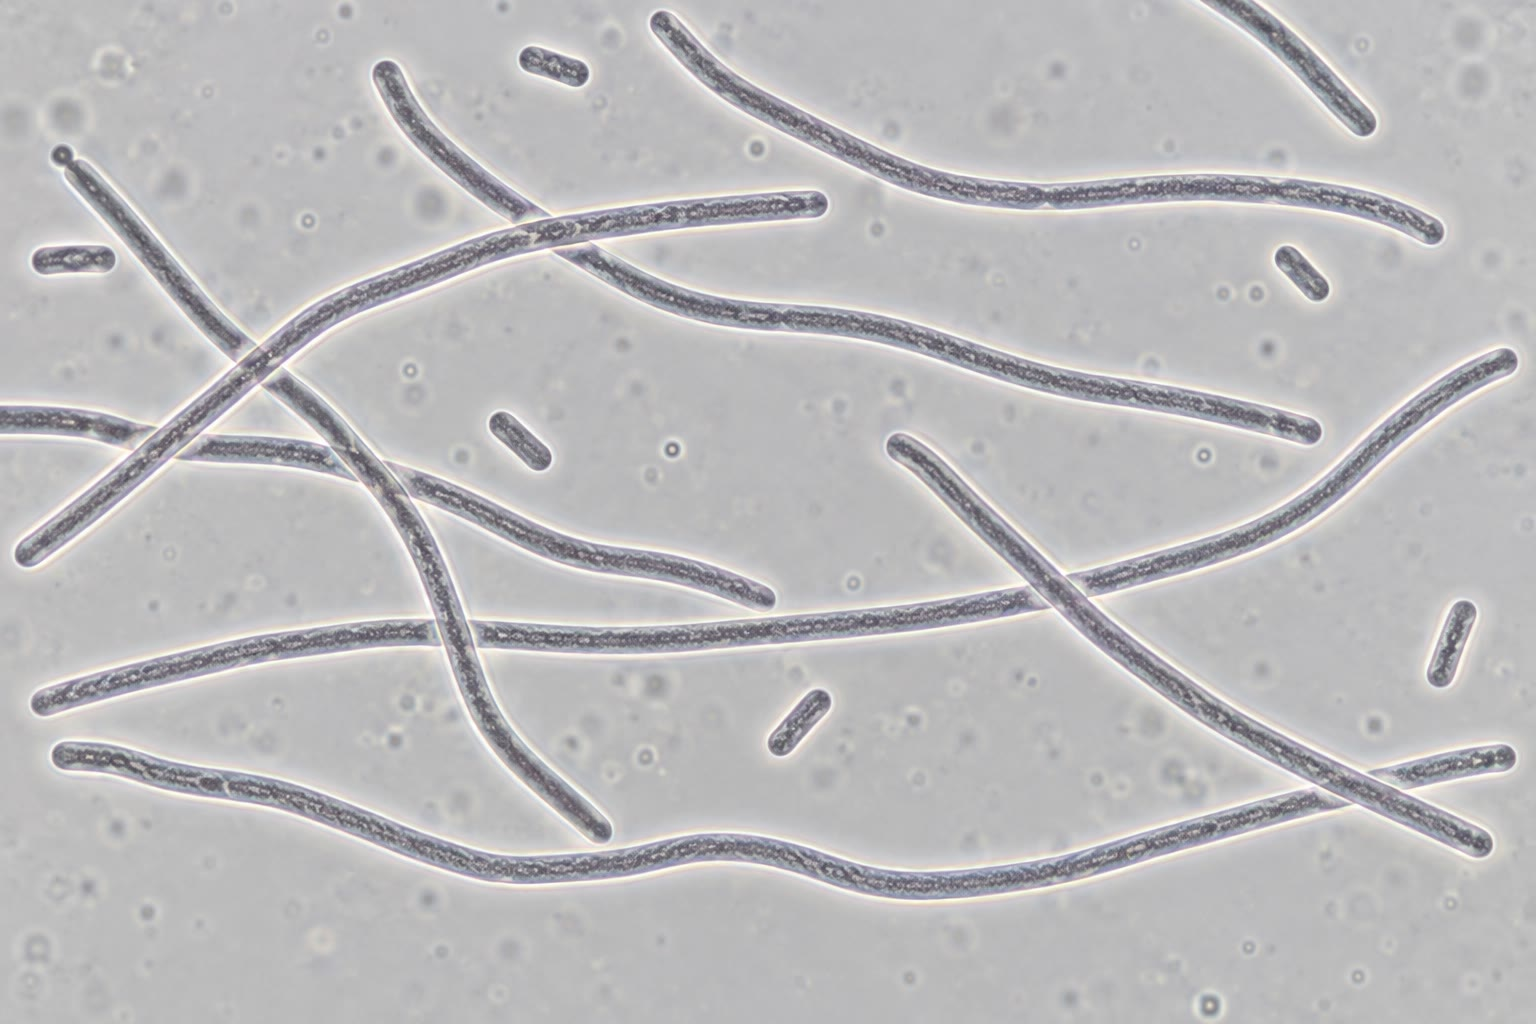
\includegraphics[width=0.46\linewidth]{images/book5/ai/b5-03-sos-filaments.jpg}\hspace{0.04\linewidth}
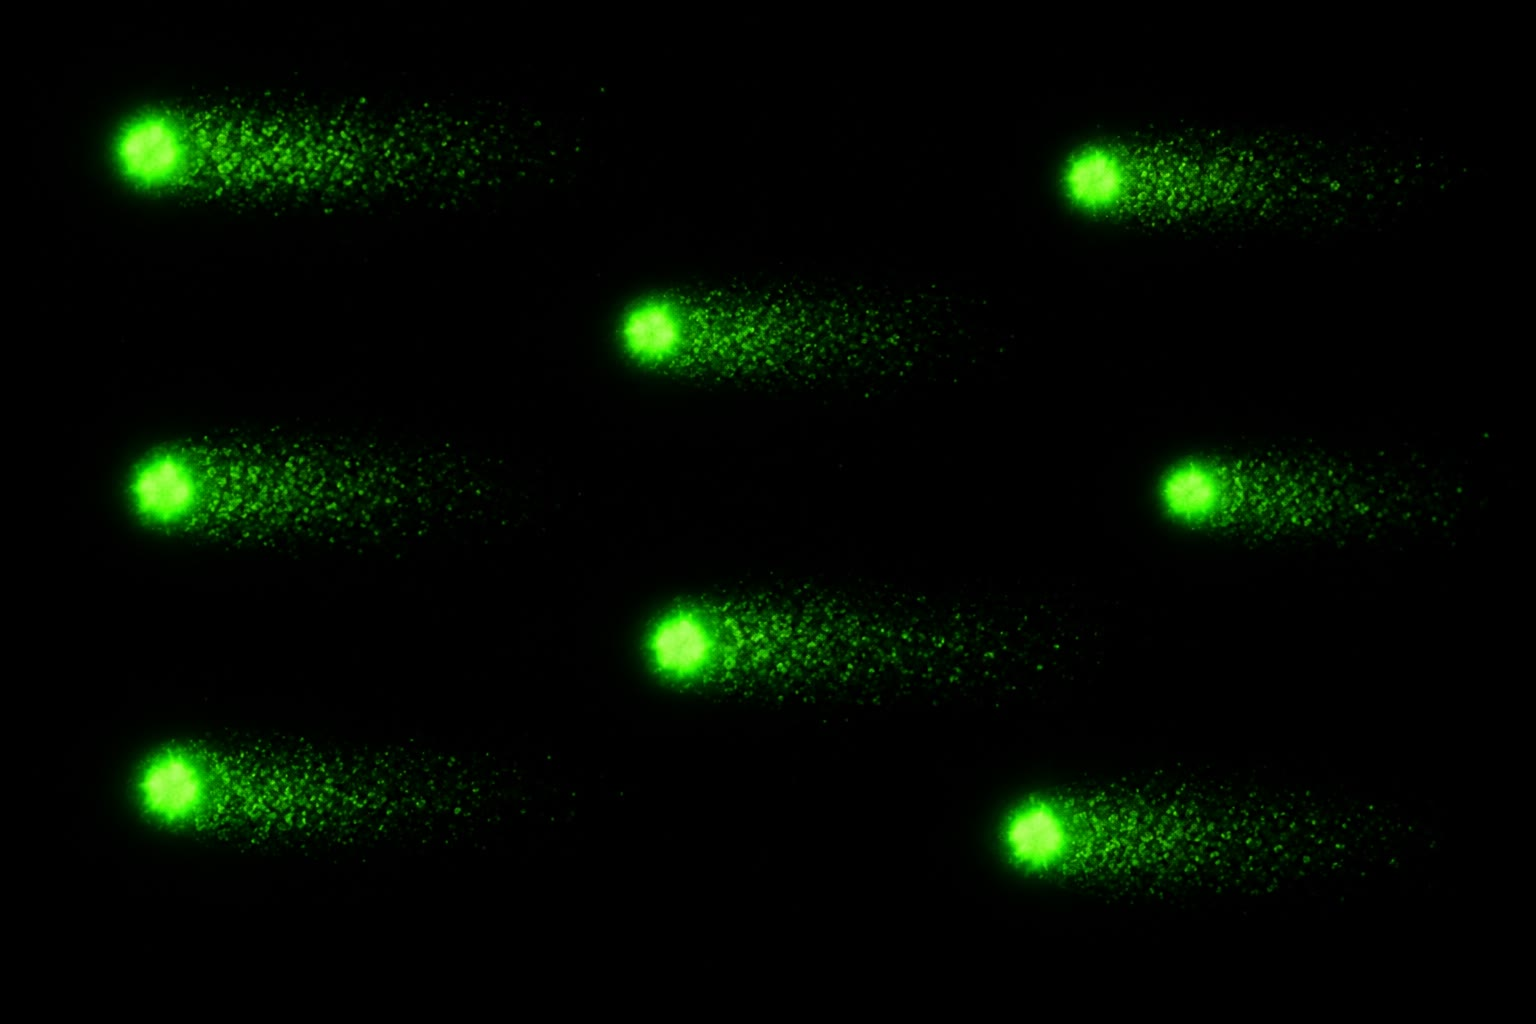
\includegraphics[width=0.46\linewidth]{images/book5/ai/b5-03-comet-assay.jpg}

{\small À esquerda: \emph{E.~coli} depois da irradiação ultravioleta,
crescida em longos filamentos porque a \omterm{prop:b3:dna-repair:sos}{resposta SOS} bloqueou a divisão
celular enquanto o DNA é reparado. À direita: um ensaio cometa ---
células isoladas embebidas num gel e submetidas a eletroforese; o DNA
fragmentado escorre para fora do núcleo numa cauda cujo comprimento
mede o número de quebras.}
\end{omfigure}

\begin{definition}[A resposta ao dano no DNA]\label{def:b3:dna-repair:ddr}
\index{resposta ao dano no DNA}\index{ATM}\index{ponto de checagem}\index{p53}\index{gama-H2AX}
Os eucariontes sinalizam o dano por duas cinases: a \emph{ATM},
recrutada pelo complexo MRN às \omterm{def:b3:dna-repair:lesions}{quebras de fita dupla}, e a \emph{ATR},
recrutada ao DNA de fita simples das forquilhas paradas. Elas
fosforilam centenas de alvos. Em minutos a \omterm{def:b3:chromatin-epigenetics:nucleosome}{histona} H2AX é fosforilada
(\emph{$\gamma$-H2AX}) ao longo de megabases em torno de cada quebra,
formando um foco que recruta as proteínas de reparo e pode ser contado
ao microscópio, um foco por quebra. As cinases Chk1 e Chk2 detêm o
ciclo celular --- os \emph{pontos de checagem} do
\cref{ch:b3:cell-cycle-apoptosis} --- ao inativar as fosfatases que
levariam à entrada em S ou em M; e o fator de transcrição \emph{p53},
estabilizado por fosforilação, induz o inibidor de cinase dependente
de ciclina p21 (uma parada duradoura em G1), genes de reparo e, se o
dano for pesado ou persistir, os genes apoptóticos que matam a célula.
A resposta compra tempo para o reparo e, quando o reparo falha, remove
a célula em vez de deixá-la dividir-se com um genoma quebrado.
\end{definition}

\begin{omfigure}
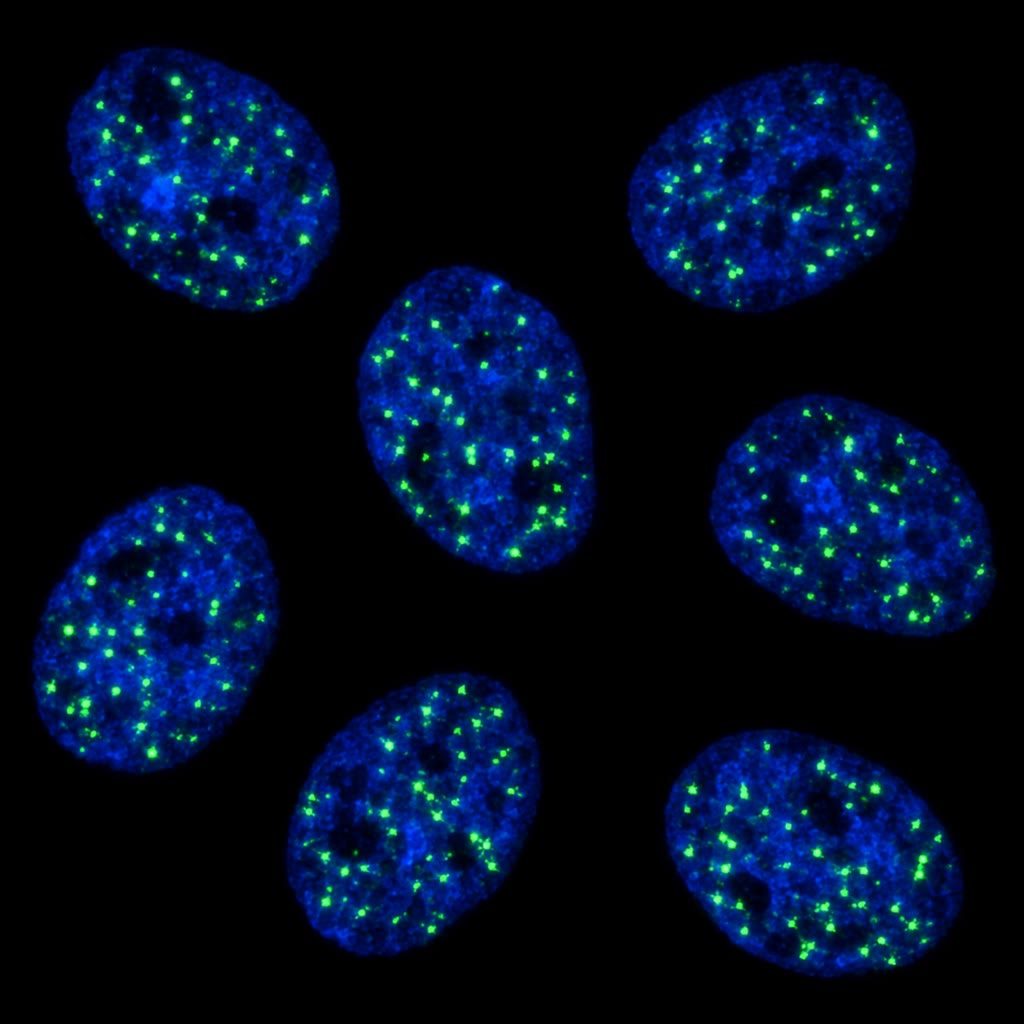
\includegraphics[width=0.4\linewidth]{images/book5/ai/b5-03-gamma-foci.jpg}

{\small Focos de $\gamma$-H2AX (verde) em núcleos (azul) uma hora após
a irradiação. Cada foco marca uma \omterm{def:b3:dna-repair:lesions}{quebra de fita dupla}; contá-los mede
o dano e, ao longo das horas seguintes, seu reparo.}
\end{omfigure}

\begin{example}[Letalidade sintética: BRCA e PARP]\label{ex:b3:dna-repair:parp}
As mulheres que herdam uma cópia defeituosa de \emph{BRCA1} ou de
\emph{BRCA2} têm um risco de câncer de mama ao longo da vida de
\qtyrange{50}{80}{\%}; os tumores surgem em células que perderam a
segunda cópia e já não conseguem fazer \omterm{def:b3:dna-repair:dsb}{recombinação homóloga}. Tais
células reparam suas \omterm{def:b3:dna-repair:lesions}{quebras de fita dupla} apenas por junção de
extremidades e acumulam rearranjos. Elas também adquirem uma fraqueza
específica. As quebras de fita simples, umas \num{10000} por dia, são
reparadas por uma rota que precisa da enzima PARP; quando a PARP é
inibida por um fármaco, as quebras de fita simples persistem até a
fase S, em que uma forquilha converte cada uma numa \omterm{def:b3:dna-repair:lesions}{quebra de fita
dupla} com apenas uma extremidade --- reparável só por recombinação.
Uma célula normal, com um alelo \emph{\omterm{def:b3:dna-repair:dsb}{BRCA}} bom, dá conta; a célula
tumoral morre. Dois defeitos, inócuos isoladamente, são letais juntos:
o fármaco mata por \emph{letalidade sintética} e poupa as demais
células da paciente.
\end{example}

\begin{proposition}[A recombinação como ferramenta]\label{prop:b3:dna-repair:tools}
\index{recombinação sítio-específica}\index{Cre-lox}
As recombinases sítio-específicas cortam e reúnem o DNA em sequências
curtas definidas, sem busca de homologia nem síntese: a enzima Cre do
fago P1 age sobre sítios \emph{loxP} de \qty{34}{bp}, a enzima Flp da
levedura sobre sítios \emph{FRT}. Dois sítios na mesma orientação
numa mesma molécula excisam o DNA entre eles como um círculo; em
orientações opostas, invertem-no; sítios em duas moléculas trocam seus
flancos. Um gene ladeado por sítios \emph{loxP} (``floxeado'') é
deletado apenas nas células em que a Cre é expressa, a partir de um
promotor à escolha do experimentador, ou no momento que o
experimentador escolher se a Cre for ativada por um fármaco: é assim
que um gene essencial ao embrião é estudado no fígado adulto, ou no
neurônio, isoladamente (\cref{ch:b3:genetic-engineering}). A própria
\omterm{def:b3:dna-repair:dsb}{recombinação homóloga} da célula é o que o direcionamento gênico e a
edição dirigida por CRISPR tomam emprestado para escrever uma
sequência escolhida num lugar escolhido.
\end{proposition}

\begin{remark}[Reparo e envelhecimento]\label{rem:b3:dna-repair:ageing}
As células que não conseguem reparar acumulam mutações, entram em
senescência ou morrem; os defeitos herdados de reparo (síndrome de
Werner, uma helicase; síndrome de Cockayne, o reparo acoplado à
transcrição; ataxia-telangiectasia, a \omterm{def:b3:dna-repair:ddr}{ATM}) causam traços de
envelhecimento precoce, e a contagem de mutações somáticas dos tecidos
normais sobe linearmente com a idade, a uma taxa de algumas dezenas de
mutações por célula por ano. Se o dano acumulado \emph{causa} o
envelhecimento comum, ou apenas o acompanha, não está resolvido; que a
capacidade de reparar seja um determinante da longevidade entre as
espécies --- as espécies mais longevas reparam mais --- está bem
apoiado.
\end{remark}

\section{Exercícios}

\begin{exercise}[$\star$]\label{exo:b3:dna-repair:1}
Classifique estas lesões como espontâneas ou ambientais e nomeie a via
de reparo de cada uma: uma uracila no DNA; um dímero de timina; uma
\omterm{def:b3:dna-repair:lesions}{8-oxoguanina}; um mau pareamento G--T atrás da forquilha; uma \omterm{def:b3:dna-repair:lesions}{quebra de
fita dupla} em G1.
\end{exercise}

\begin{exercise}[$\star$]\label{exo:b3:dna-repair:2}
Por que o \omterm{def:b3:dna-repair:excision}{reparo por excisão de nucleotídeos} não precisa de uma enzima
específica para cada tipo de \omterm{def:b3:dna-repair:lesions}{lesão}, ao passo que o \omterm{def:b3:dna-repair:excision}{reparo por excisão
de bases} precisa de uma \omterm{def:b3:dna-repair:excision}{glicosilase} para cada uma?
\end{exercise}

\begin{exercise}[$\star$]\label{exo:b3:dna-repair:3}
Enuncie o problema da discriminação de fitas no \omterm{prop:b3:dna-repair:fidelity}{reparo de mau
pareamento} e como \emph{E.~coli} o resolve. O que aconteceria num
mutante \emph{dam}, que não metila nenhum sítio GATC?
\end{exercise}

\begin{exercise}[$\star$]\label{exo:b3:dna-repair:4}
Uma célula recebe \qty{2}{Gy} de raios X. Quantas \omterm{def:b3:dna-repair:lesions}{quebras de fita
dupla} ela sofre, grosso modo, e quantos focos de $\gamma$-H2AX você
esperaria contar uma hora depois? Por que menos após seis horas?
\end{exercise}

\begin{exercise}[$\star\star$]\label{exo:b3:dna-repair:5}
Usando a \cref{prop:b3:dna-repair:fidelity}, calcule a taxa de mutação
por par de bases e o número de mutações novas por genoma diploide por
divisão em (a) uma célula normal, (b) uma célula sem \omterm{prop:b3:dna-repair:fidelity}{reparo de mau
pareamento}, (c) uma célula cuja polimerase perdeu sua exonuclease.
Qual é a mutadora mais perigosa?
\end{exercise}

\begin{exercise}[$\star\star$]\label{exo:b3:dna-repair:6}
Sítios abásicos surgem a $10^{4}$ por célula por dia e são reparados
com meia-vida de \qty{15}{min}. Use o \cref{thm:b3:dna-repair:load}
para achar o número estacionário de sítios abásicos numa célula. Se um
fármaco desacelera o reparo dez vezes, qual é o novo estado
estacionário, e quantos sítios uma forquilha encontraria se copiasse o
genoma em \qty{8}{h}?
\end{exercise}

\begin{exercise}[$\star\star$]\label{exo:b3:dna-repair:7}
Em G2 uma quebra pode ser reparada por NHEJ (meia-vida \qty{30}{min})
ou por HR (meia-vida \qty{4}{h}), ambas disponíveis. Que fração das
quebras vai pela HR? Qual é a meia-vida das quebras? Por que a HR é,
ainda assim, a via que importa nas forquilhas de replicação colapsadas?
\end{exercise}

\begin{exercise}[$\star\star$]\label{exo:b3:dna-repair:8}
Preveja o comportamento dos microssatélites, o espectro de tumores e a
sensibilidade à luz do sol de um paciente com (a) \omterm{def:b3:dna-repair:mmr}{síndrome de Lynch},
(b) \omterm{def:b3:dna-repair:excision}{xeroderma pigmentoso} do grupo~A, (c) a variante XP-V, sem a
Pol~$\eta$.
\end{exercise}

\begin{exercise}[$\star\star$]\label{exo:b3:dna-repair:9}
Dois sítios \emph{loxP} na mesma orientação ladeiam o éxon~3 de um
gene; a Cre é expressa a partir de um promotor ativo apenas no fígado
desde o nascimento. Descreva o genótipo das células hepáticas e o dos
neurônios no adulto, e o que acontece se os sítios forem postos em
orientações opostas.
\end{exercise}

\begin{exercise}[$\star\star\star$]\label{exo:b3:dna-repair:10}
Explique por que a \omterm{prop:b3:dna-repair:sos}{resposta SOS} liga os genes de reparo antes das
polimerases propensas a erro, usando as afinidades da LexA por seus
operadores, e por que uma bactéria desprovida das polimerases
propensas a erro poderia mesmo assim estar em desvantagem num paciente
tratado com antibióticos.
\end{exercise}

\begin{exercise}[$\star\star\star$]\label{exo:b3:dna-repair:11}
Um inibidor de PARP mata células tumorais deficientes em \emph{\omterm{def:b3:dna-repair:dsb}{BRCA}},
mas não as células normais da paciente. Exponha a cadeia causal e, em
seguida, preveja dois modos pelos quais um tumor poderia tornar-se
resistente ao fármaco e como você detectaria cada um.
\end{exercise}

\begin{exercise}[$\star\star\star$]\label{exo:b3:dna-repair:12}
A conversão gênica numa permuta dá tétrades $3{:}1$. Desenhe (ou
descreva) uma \omterm{def:b3:dna-repair:dsb}{junção de Holliday} com um heterodúplex que abranja um
marcador, e mostre como o \omterm{prop:b3:dna-repair:fidelity}{reparo de mau pareamento} do heterodúplex num
sentido dá $3{:}1$, no outro dá $1{:}3$, e a ausência de reparo dá um
esporo ele próprio heterozigoto (uma segregação pós-meiótica). Por que
a conversão se restringe a marcadores próximos da permuta?
\end{exercise}

\section{Problema: um dia na vida de um genoma}

\begin{problem}[{Problema de fim de semana --- o dano diário de uma
célula humana contado, a escada da fidelidade multiplicada, uma dose
de sol acompanhada até a forquilha numa célula normal e numa
deficiente em reparo, uma dose de raios X repartida entre duas vias de
reparo e a fraqueza de um tumor convertida em fármaco, terminando no
número de dímeros que a forquilha encontra, na taxa de mutação por
base e na fração de quebras que a recombinação repara}]
\label{pb:b3:dna-repair:1}
Dados: uma célula humana diploide tem $6.4\times 10^{9}$ bp,
\qty{1.5}{\%} deles codificadores de proteína. Dano espontâneo por
dia: $10^{4}$ depurinações, $400$ desaminações de citosina, $10^{4}$
quebras de fita simples. Fidelidade: polimerase $10^{-5}$, a revisão
deixa $10^{-2}$ dos erros, o \omterm{prop:b3:dna-repair:fidelity}{reparo de mau pareamento} $10^{-3}$. Um
banho de sol deixa $10^{5}$ \omterm{def:b3:dna-repair:lesions}{dímeros de pirimidina} por célula da pele;
o reparo por excisão tem meia-vida de \qty{2}{h} normalmente e de
\qty{70}{h} no \omterm{def:b3:dna-repair:excision}{xeroderma pigmentoso}; uma forquilha chega \qty{8}{h}
depois; o contorno de um dímero pela translesão causa uma mutação com
probabilidade $10^{-3}$. Os raios X produzem $35$ \omterm{def:b3:dna-repair:lesions}{quebras de fita
dupla} por gray; meia-vida da NHEJ \qty{30}{min}, da HR \qty{4}{h}.

\medskip
\noindent\textbf{Parte I --- Dias comuns.}
\begin{enumerate}
  \item Quantas lesões espontâneas a célula sofre por dia, e por ano?
        Compare com o tamanho do genoma.
  \item Calcule a taxa de mutação por par de bases por divisão e o
        número esperado de mutações novas por divisão.
  \item Quantas delas caem em sequência codificadora de proteína? Ao
        longo das cerca de $50$ divisões do zigoto a uma célula de
        pele adulta, quantas mutações codificadoras uma célula da pele
        carrega só pela replicação?
  \item Uma célula sem \omterm{prop:b3:dna-repair:fidelity}{reparo de mau pareamento}: taxa de mutação e
        mutações por divisão? Um microssatélite desliza uma vez em
        $10^{4}$ divisões sem \omterm{prop:b3:dna-repair:fidelity}{reparo de mau pareamento} e uma vez em
        $10^{7}$ com ele. Num tumor de $10^{9}$ células derivadas por
        $40$ divisões, quantas células carregam um alelo deslizado num
        dado microssatélite em cada caso? (Estime com taxa $\times$
        divisões $\times$ células.)
  \item A \omterm{def:b3:dna-repair:lesions}{desaminação} da citosina dá uracila, a da 5-metilcitosina dá
        timina. Qual é reparada, por quê, e qual se torna mutação?
        Relacione com o déficit de \omterm{def:b3:chromatin-epigenetics:methylation}{CpG} do
        \cref{ch:b3:chromatin-epigenetics}.
  \item Uma guanina oxidada (8-oxoG) pareia com A durante a
        replicação. A célula tem uma \omterm{def:b3:dna-repair:excision}{glicosilase} para a 8-oxoG em
        frente a C, outra para o A em frente à 8-oxoG e uma hidrolase
        que destrói o dGTP oxidado. Explique o que cada uma previne e
        que mutação resulta quando as três falham.
\end{enumerate}

\medskip
\noindent\textbf{Parte II --- Um dia ao sol.}
\begin{enumerate}[resume]
  \item Calcule as constantes de taxa de excisão $k$ da célula normal
        e da célula XP.
  \item Quantos dímeros restam na forquilha em cada uma?
  \item Quantas mutações o banho de sol causa por célula em cada caso,
        e quantas delas estão em sequência codificadora?
  \item Ao longo de uma infância de $500$ exposições dessas, quantas
        mutações codificadoras por célula da pele em cada caso?
        Compare com o número devido apenas à replicação da questão 3.
  \item Cerca de $20$ genes, somando \qty{40}{kb} de sequência
        codificadora, podem impulsionar um câncer de pele quando
        mutados. Qual é a probabilidade, por célula, de ao menos uma
        mutação induzida pelo banho de sol cair num deles, na criança
        com XP? (Use uma Poisson com a média certa.) Com $10^{9}$
        células expostas, quantas são atingidas?
  \item Explique por que o problema das células XP é da forquilha, e
        não da \omterm{def:b3:dna-repair:lesions}{lesão} em si, e por que os cânceres aparecem só na pele.
\end{enumerate}

\medskip
\noindent\textbf{Parte III --- Uma dose de raios X.}
\begin{enumerate}[resume]
  \item Uma dose de \qty{2}{Gy}: quantas \omterm{def:b3:dna-repair:lesions}{quebras de fita dupla}, e
        quantos focos de $\gamma$-H2AX após uma hora se a NHEJ for a
        única via (célula em G1)?
  \item Numa célula em G2 as duas vias operam. Calcule as constantes
        de taxa e a fração de quebras reparadas pela HR.
  \item Qual é a meia-vida das quebras em G2, e quantas restam após
        uma hora?
  \item Cada evento de NHEJ altera alguns pares de bases na junção. Se
        uma junção cai em sequência codificadora com probabilidade
        $0.015$ e a alteração então rompe o gene com probabilidade
        $0.7$, quantos genes a dose de \qty{2}{Gy} rompe por célula em
        G1?
  \item Com $n$ quebras simultâneas, as extremidades podem ser unidas
        erradas numa translocação. Suponha que cada um dos $n(n-1)/2$
        pares de quebras seja unido de modo errado com probabilidade
        $3\times 10^{-4}$. Translocações esperadas por célula a
        \qty{2}{Gy}? E a \qty{0.2}{Gy}? Por que o risco escala com o
        quadrado da dose enquanto o número de quebras escala
        linearmente?
  \item A mesma dose de \qty{2}{Gy} dada ao longo de \qty{10}{h} em
        vez de num instante: quantas quebras estão presentes ao mesmo
        tempo (estado estacionário, NHEJ)? O que isso implica para as
        translocações e para a prática de fracionar a radioterapia?
  \item Uma célula sobrevive a uma dose $D$ com probabilidade
        $e^{-D/D_{0}}$, com $D_{0} = \qty{1.5}{Gy}$ para uma célula de
        reparo intacto e \qty{0.5}{Gy} para uma sem NHEJ. Calcule a
        sobrevivência de cada uma a \qty{2}{Gy} e a \qty{6}{Gy}, e
        interprete $D_{0}$.
\end{enumerate}

\medskip
\noindent\textbf{Parte IV --- A fraqueza do tumor.}
\begin{enumerate}[resume]
  \item Uma célula tumoral deficiente em \emph{BRCA2} repara as
        quebras só por NHEJ. Usando a questão 14, que fração de suas
        quebras em S/G2 passa a ser reparada de modo inacurado, quando
        uma célula normal a repararia de modo acurado? O que isso faz
        a seu genoma ao longo dos anos?
  \item A inibição da PARP deixa as $10^{4}$ quebras diárias de fita
        simples sem reparo; \qty{1}{\%} delas é convertido pelas
        forquilhas em \omterm{def:b3:dna-repair:lesions}{quebras de fita dupla} com uma só extremidade.
        Quantas quebras dessas por dia por célula, e por que a NHEJ
        não consegue reparar corretamente uma quebra de uma só
        extremidade?
  \item Explique por que as células normais da paciente, heterozigotas
        para \emph{BRCA2}, sobrevivem ao fármaco.
  \item Um tumor torna-se resistente por uma segunda mutação que
        restaura a fase de leitura de \emph{BRCA2}. Explique e diga
        como você o detectaria.
  \item A quimioterapia com um agente alquilante mata as células
        tumorais por meio do \omterm{prop:b3:dna-repair:fidelity}{reparo de mau pareamento}: a enzima tenta
        reparar as bases alquiladas e dispara a morte celular. Preveja
        o efeito do fármaco sobre um tumor de \omterm{def:b3:dna-repair:mmr}{síndrome de Lynch}, que
        não tem \omterm{prop:b3:dna-repair:fidelity}{reparo de mau pareamento}.
  \item Enuncie os três resultados: os dímeros encontrados pela
        forquilha na célula XP (questão~8), a taxa normal de mutação
        por par de bases (questão~2) e a fração de quebras em G2 que a
        HR repara (questão~14).
\end{enumerate}
\end{problem}
